\section{Dokumentation}
\subsection{Forklar hvad arv er}

Et af de vigtigste elementer i objektorienteret programmering er nedarvning, men hvad betyder nedarvning? At arve betyder i bund og grund at noget med en materiel værdi overdrages til noget eller nogle efterkommere. I programmerings verden ville man hellere definere arv som en eller flere egenskaber der overføres fra en generation til en anden generation, også sagt på en anden måde, at en klasse der får overført egenskaber fra en anden klasse. Den klasse der nedarves fra kaldes for en Superklasse (parent), hvor klassen der nedarver eller får egenskaber fra en Superklasse, kaldes for en Subklasse (child).
Ved benyttelse af denne proces vil oplysningerne om de forskellige klasser ende op i en hierarkisk rækkefølge. 
På figur 7 ses forskellige eksempler på typer af nedarvning der findes, men dog skal man være opmærksom på, at Java ikke understøtter flere nedarvninger. I Java kan en klasse kun have én Superklasse, dvs. at hver klasse kun kan nedarve fra én klasse. \footnote{ Java Programmering - En bog for begyndere af Henrik Kressner}

\begin{figure}[h]\label{fig:types_of_inheritance.jpg} 
    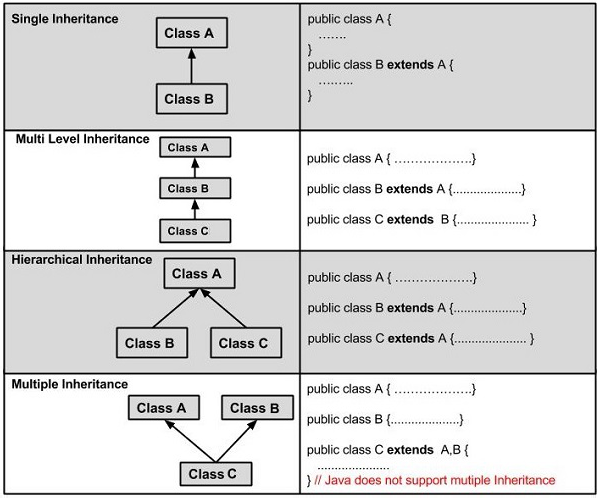
\includegraphics[width=8cm]{fig/types_of_inheritance.jpg}
    \caption{eksempel på typer af arv}
\end{figure}
%\footnote{https://www.tutorialspoint.com/java/java_inheritance.htm}
\subsection{Forklar hvad abtract betyder}
Den abstrakte klasse kører ingen metoder, og indeholder kun attributter. Klassen bruges som en slags ”over”-klasse, hvor andre klasser nedarver attributterne. Det anvendes i en situation, hvor man f.eks har to klasser, der har mange af de samme attributter. Så vil alle de attributter, som de har tilfælles stå i den abstrakte klasse.
Hvis man f.eks har klasserne lærer og elev, kunne den abstrakte klasse til disse, hedde ”personer”, da både lærer og elever har en fødselsdato, køn, navn osv.

\subsection{Fortæl hvad det hedder hvis alle fieldklasserne har en landOnField metode der gør noget forskelligt}

% IOException: Sentence length out of bounds.

Hvis alle fieldklasserne gør brug af den samme landOnField metode, er det fordi, denne metode er en super metode. En super metode er nedarvet til de forskellige subklasser fra super klassen, dette gør at alle klasserne kan gøre brug af samme metode. Eksempeltvis, hvis vi har en masse dyr som klasser, kat, hund, kanin etc. så kan de alle nedarve super metoden eat() fra 
superklassen som hedder SurvivalRequirements, eftersom disse er metoder alle dyrene får brug for, så vil det give mening at lave det til en superklasse med supermetoder, så der holdes lav kobling og høj kohæsion, samt undgås kopiring af kode og høj mulighed for genbrug.

\subsection{Dokumentation for test med screenshots}
    \subsection{JUnit test}
        JUnit test er en autonomisreret testmetode. Her skriver/koder man selv en test, som tester java kode. Oftest opbygger man JUnit test ud fra Java klasser.
        Der er mange måder, hvorpå man kan bruge JUnit testen. Man kan både skrive testen inden, man kan skrive den efter, man kan lave den på baggrund af indsigt i koden eller uden nogen form til kendskab af programkoden. Det to sidst nævnte kaldes Black- og Whitebox test.

        Her er et eksempel på et stykke udført JUnit test fra vores spil:
            \begin{figure}[h]\label{fig:JunitTest.jpg}
                \advance\leftskip-3cms
                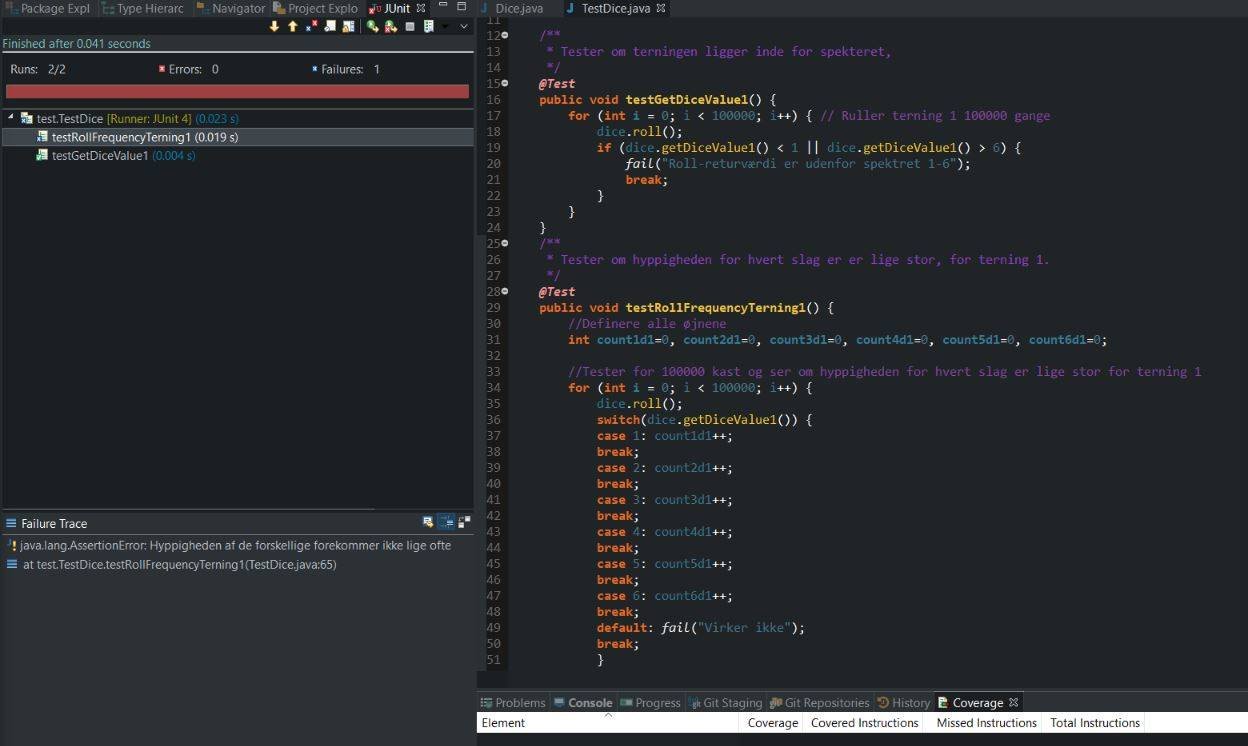
\includegraphics[width=20cm]{fig/JunitTest.jpg}
                \caption{JUnit test udført i Eclipse den 23/11-2017}
            \end{figure}
        Det ser på Figur \ref{fig:JUnitTest} at koden ikke bestod testen, hvor vi også får vist den rette, selv skrevet, fejl besked.

    \subsection{Positiv negativ test}
        Denne test bruges for at teste om systemet kan håndterer 'ugyldige' input, dette kan både være negative som positive værdier, såvel som bogstaver og andre tegn. Denne test forbindes oftest med en eller flere ækvivalensklasse test.
    \subsection{Black- og Whitebox test}

    \textbf{Blackbox test}: Her har man intet kendskab til koden, ud over hvad denne skal kunne gøre. Det er derfor lige til højrebenet, at teste det faktiske output mod det forventede output og at teste ækvivalensklasserne.
    \textbf{Whitebox test}: Her opstiller man tests på baggrund af koden og dens opbygning. Man vil med disse tests teste hele koden, altså alle instruktioner, forgreninger og stier, som koden kan blive udført i. Dette er ikke altid muligt med \textit{BlackBox testen}, da man her, ikke har et indblik i koden.
   
\subsection{Dokumentation for overholdt GRASP}
GRASP står for \textit{General Responsibility Assignment Software Patterns}. 
GRASP bruges til at give det rigtige ansvar til de forskellige klasser, 
der bliver oprettet under udviklingen af et program. GRASP indeholder 9 patterns. 
Patterns bliver brugt til at strukturere et problem, samt at finde en passende løsning. De 9 patterns er:
    \begin{enumerate}
        \item Creator
        \item Information expert
        \item Low coupling
        \item Controller
        \item High cohesion
        \item Indirection
        \item Polymorphism
        \item Protected variations
        \item Pure fabrication
    \end{enumerate}
Disse patterns kan bruges som guidelines til at udvikle et software projekt.
Her løser man problemer som ofte opstår under software udvikling, ved at gøre det overskueligt hvilken
class der har ansvar for hvad. Vores Creator class er "GameController" som sørger for at "Player" class'ens
information går videre til selve spillet. Information Expert er vores "Player" class, 
da den indeholder antallet af spillere
og deres brikker.


\subsection{Vejledning til import af Git Repository til eclipse}
Man skal i første omgang have et URL af det pågældende repository, som du kopierer.
Derefter åbner du eclipse og åbner menuen 
Window $\Rightarrow$ View $\Rightarrow$ søg på "git" $\Rightarrow$ git repositories.
Derefter har du vinduet "Git Repositories", hvor der er en knap; "Clone a git repository and add to this view".
Ikonet er mappen i midten med en blå pil på, her trykker du.
Hvis du huskede at kopiere URL'et trykker du nu "Next", hvorefter at alle branches bliver loaded. Når den har loaded trykker du next igen.
Nu kommer du til det sidste vindue, hvor du trykker "Finish, og nu har du importeret(clonet) git repositoriet.

\subsection{Brugertests}

\begin{center}
    \begin{tabular}{ | {1cm} | m{2cm}| m{2cm}| m{5cm}| m{5cm}| {1cm} }
            \hline
                Test person & Hvad man vil teste & Trin & Forventet resultat & Testresultat\\
            \hline
                Spillere & Antallet af spillere & Vælg antallet af spillere & Man kan være mellem 2 - 4 spillere & Pass  \\
            \hline
                Spillere & Går turen videre & Spillerne slår med terningerne & En spiller slår med terningerne og turen går videre efter & Pass \\
            \hline
                Spillere & Udskrives der tekst når en spiller lander på et felt & Når en spiller lander på et felt & Der bliver printet en tekst der fortæller om feltet & Pass \\
            \hline
                Spillere & Køber spilleren feltet når han/hun lander på det & Når spillet er i gang & Feltet bliver opkøbt & Pass \\
            \hline
                Spillere & Spilleren er tvunget til at betale ejeren af feltet han lander på & Når spillet er i gang & Spilleren betaler ham/hende der ejer feltet & Pass \\
            \hline
        \end{tabular}
\end{center}           
\pagebreak 
\begin{center}
    \begin{tabular}{ | {1cm} | m{3cm}| m{2cm}| m{5cm}| m{5cm}| {1cm} }
                      
            \hline
                Spillere & Får spilleren 2M når de passere start feltet & Når spillet er i gang & Spillerens balance stiger med 2M & Pass \\
            \hline
                Spillere & Ryger spilleren i fængsel og mistes der 2M & Når en spiller lander på "FÆNGSEL" & Spilleren modtager ikke 2M & Pass \\
            \hline
                Spillere & Skal spilleren give sit omkostningskort eller betale 1M når han/hun er i fængsel & Når en spiller er på "FÆNGSEL" feltet & Spillerens mister sit omkostningskort eller betaler 1M hvis kortet er brugt & Fail \\
            \hline
                Spillere & Virker chancekort & Når en spiller trækker et chancekort & Spilleren trækker et chancekort og får en effekt & Fail \\
            \hline
            %12. krav
                Spillere & Virker besøg feltet & Når en spiller lander på "Besøg" feltet & Der sker intet og turen går videre & Pass \\
        
        \hline
            %16. krav
        Spillere & Kan spillerne gå rundt om pladen & Når spillerne har været en runde rundt på pladen & Spillerne kan gå flere omgange rundt på pladen & Pass \\
        \hline
    \end{tabular}
\end{center}
\pagebreak
        \begin{center}
\begin{tabular}{ | {1cm} | m{2cm}| m{2cm}| m{5cm}| m{5cm}| {1cm} }
\\          Spiller & slutter spillet, når den første spiller går bankerot & kører spillet indtil en spiller har nul eller færre M.& Spillet slutter & Pass \\
        \hline
            Spiller & Sker der ingenting, og turen gives videre, hvis man lander på "gratis parkering" & Spiller indtil man rammer "Gratis parkering" & Ingenting sker og turen går videre & Pass \\
        \hline    
            Spiller & Printes der "Tillykke (spiller), du har vundet", når spillet sluttes & kører spillet indtil en spiller har nul eller færre M. & Der bliver printet den ønskede tekst & Pass \\
        \hline    
            Spiller & Kan spillet spilles på DTU's databarer & åbner spillet på computeren & Spillet køres & pass \\
        \hline
    \end{tabular}
\end{center}